\documentclass[../talk.tex]{subfiles}
\begin{document}

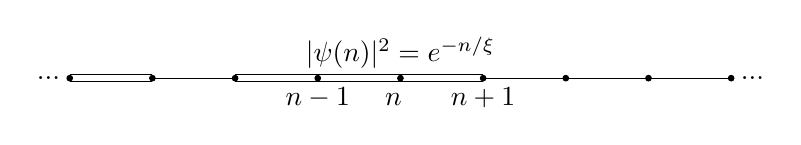
\begin{tikzpicture}[scale=.7]
    		\newcommand{\orig}{-1.5}
    		\newcommand{\trans}{1.5}
    		\newcommand{\vertspac}{-2.}
    		 \newcommand{\rad}{2pt} % radii of the circles
    		     		
    		% set the style of the strong bonds
    		\tikzset{
    			strong/.style={
    				double,
    				double distance=\rad,
    				line width=0.5pt
    				}
    		}
    	
    		% bonds 
        	\draw[strong] (\orig+\trans,0) -- (\orig+2*\trans,0) node [midway, above] {};
			\draw[-] (\orig+2*\trans,0) -- (\orig+3*\trans,0) node [midway, above] {};	
			\draw[strong] (\orig+3*\trans,0) -- (\orig+4*\trans,0) node [midway, above] {};
			\draw[strong] (\orig+4*\trans,0) -- (\orig+5*\trans,0) node [midway, above] {};
			\draw[strong] (\orig+5*\trans,0) -- (\orig+6*\trans,0) node [midway, above] {};
			\draw[-] (\orig+6*\trans,0) -- (\orig+7*\trans,0) node [midway, above] {};
			\draw[-] (\orig+7*\trans,0) -- (\orig+8*\trans,0) node [midway, above] {};
			\draw[-] (\orig+8*\trans,0) -- (\orig+9*\trans,0) node [midway, above] {};
    	
    		% sites
		    \filldraw (\orig+1*\trans,0) circle (0.05) node [left] {...};
		    \filldraw (\orig+2*\trans,0) circle (0.05) node [below] {};
		    \filldraw (\orig+3*\trans,0) circle (0.05) node [below] {};
		    \filldraw (\orig+4*\trans,0) circle (0.05) node [below] {$n-1$};
		    \filldraw (\orig+5*\trans,0) circle (0.05) node [below] {$n\phantom{1}$} node [above] {$|\psi(n)|^2 = e^{- n/\xi}$};
		    \filldraw (\orig+6*\trans,0) circle (0.05) node [below] {$n+1$};
		    \filldraw (\orig+7*\trans,0) circle (0.05) node [below] {};
		    \filldraw (\orig+8*\trans,0) circle (0.05) node [right] {};
		    \filldraw (\orig+9*\trans,0) circle (0.05) node [right] {...};
		      
		\end{tikzpicture}
\end{document}